\documentclass[10pt,a4paper]{article}
\usepackage[T1]{fontenc}
\usepackage{tikz}
\usepackage[margin=1cm]{geometry}
\usetikzlibrary{calc,shapes.multipart,chains,arrows,positioning}
\tikzset{list/.style={very thick, rectangle split, rectangle split parts=3, draw, rectangle split horizontal, minimum size=18pt, inner sep=5pt, text=black, rectangle split part fill={blue!20, red!20, blue!20}}, ->, start chain=going right, very thick}
\begin{document}
\section*{Doubly Linked List Before Insertion}
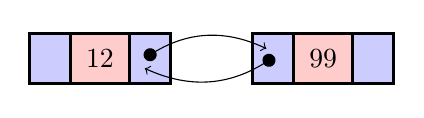
\begin{tikzpicture}
    \node[list,on chain] (N1) {\nodepart{second} 12};
    \node[list,on chain] (N2) {\nodepart{second} 99};
    \path[*->] let \p1 = (N1.three), \p2 = (N1.center) in (\x1,\y2) edge [bend left] ($(N2.one)+(0,0.2)$);
    \path[*->] ($(N2.one)+(0.1,0.1)$) edge [bend left] ($(N1.three)+(0,-0.05)$);
\end{tikzpicture}
\section*{Doubly Linked List After Insertion}
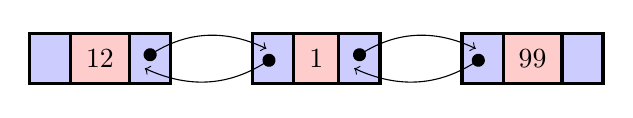
\begin{tikzpicture}
    \node[list,on chain] (N1) {\nodepart{second} 12};
    \node[list,on chain] (N2) {\nodepart{second} 1};
    \node[list,on chain] (N3) {\nodepart{second} 99};
    \path[*->] let \p1 = (N1.three), \p2 = (N1.center) in (\x1,\y2) edge [bend left] ($(N2.one)+(0,0.2)$);
    \path[*->] ($(N2.one)+(0.1,0.1)$) edge [bend left] ($(N1.three)+(0,-0.05)$);
    \path[*->] let \p1 = (N2.three), \p2 = (N2.center) in (\x1,\y2) edge [bend left] ($(N3.one)+(0,0.2)$);
    \path[*->] ($(N3.one)+(0.1,0.1)$) edge [bend left] ($(N2.three)+(0,-0.05)$);
\end{tikzpicture}
\end{document}